\documentclass{instrukcja}        
\usepackage[polish]{babel}
\usepackage[utf8]{inputenc}
\usepackage[OT4]{fontenc}

\begin{document}

\materialnumber{4}
\course[Info I]{Informatyka I}
\material[Lab 4]{Instrukcja 4}
\author{W. Regulski}
\materialtitle

\section*{Liczby losowe}
Generacja liczb losowych jest bardzo przydatna w wielu obszarach począwszy od komputerowych gier w kości a na skomplikowanych symulacjach mechanicznych i kryptografii skończywszy.
Poniższe zadania przedstawiają mechanizm generacji liczb pseudolosowych w języku C/C++\footnote{Mówimy, że generowane liczby są pseudolosowe, gdyż niemożliwe jest wygenerowanie prawdziwie losowego ciągu liczb. W praktyce świetnym źródłem ciągów liczb losowych są dane uzyskiwane z natury  np. dane meteorologiczne (www.random.org).}.\newline

Generatory liczb pseudolosowych wymagają zastosowania tzw. ziarna czyli liczby, która posłuży do inicjalizacji procesu losowania kolejnych liczb. Zazwyczaj do inicjalizacji generatora używa się czasu sczytywanego z procesora komputera, więc konieczne będzie dołączenie biblioteki {\tt time.h}\newline
Poniższy program generuje losową liczbę całkowitą z przedziału 0 do RAND\_MAX. RAND\_MAX jest zdefiniowane w bibliotece {\tt stdlib.h}, jest ono postaci \(2^{n-1}\)  np. 32767.

\begin{verbatim}
#include <stdio.h>
#include <math.h>
#include <stdlib.h>
#include <time.h>

void main()
{
     int i;

     srand ( time(NULL) );        //inicjalizacja generatora
     i = rand();                  //funkcja losująca liczbę
     printf(" Wylosowana liczba to %d\n", i);
}
\end{verbatim}

\subsection*{Ćwiczenia}
\begin{enumerate}
\item Wykonaj powyższy program kilka razy z rzędu. Co możesz powiedzieć o wyniku? 
\item Zastąp ziarno generatora {\tt  time(NULL)} stałą liczbą. Co się wówczas stanie?
\item Zmodyfikuj program tak, by losował ciąg 40 liczb psedudolosowych i wypisywał je na ekran.
\item Wypisz na ekran wartość RAND\_MAX.
\end{enumerate}

Zazwyczaj interesuje nas konkretny przedział liczb. Aby określić kres dolny oraz długość takiego przedziału musimy dokonać kilku transformacji na wylosowanych liczbach:\newline
Po prostu bierzemy  wyłącznie resztę z dzielenia przez zadaną długość przedziału i dodajemy kres dolny jak w poniższym fragmencie kodu:

\begin{verbatim}
//  kod losuje liczby z przedzialu [ 20 do 50 ]
	
	int min = 20;
	int max = 50;
	int L = max - min + 1;

	i = rand()%L + min;
\end{verbatim}

operator \% liczy resztę z dzielenia jednej liczby przez drugą. Tutaj, licząc resztę z dzielenia wyniku losowania przez 31,  otrzymujemy liczbę z przedziału 0 do 30.\newline 
\subsection*{Uwaga}
Czy taki wzór będzie generował liczby losowe o rokładzie równomiernym? W domu zastanów się nad lepszym rozwiązaniem, a poniżej wykorzystaj to najprostsze.
\subsection*{Ćwiczenia}
\begin{enumerate}
\item Zmodyfikuj powyższy program tak, aby generował liczby z przedziału od 0 do 100.
\item Wybierz krótki przedział (rzędu kilku możliwych do wylosowania liczb) i wykonaj 1000 oraz 10000 losowań. W obu przypadkach zliczaj, ile razy wylosowano każdą liczbę.
\item Wynik (informację o tym, ile razy wylosowano każdą z wartości) wydrukuj na ekranie. Co możesz powiedzieć o rozkładzie tego losowania?
\end{enumerate}

\section*{Liczby losowe typu rzeczywistego, rzutowanie}
Do tej pory losowane liczby były liczbami całkowitymi. Często potrzebujemy liczb zmiennoprzecinkowych. W tym celu po prostu przeskalujemy wylosowaną liczbę tak, aby zawsze należała do przedziału 0-1. Wystarczy podzielić wylosowaną liczbę przez RAND\_MAX. Dodatkowo należy pamiętać, że wylosowana liczba jest typu całkowitego {\tt int}, więc dzielenie przez RAND\_MAX da nam zazwyczaj 0. Aby tego uniknąć, musimy przekonwertować typ {\tt int} na typ zmiennoprzecinkowy 
{\tt double}. Taką operację nazywamy rzutowaniem. Rzutowanie ma bardzo szerokie zastosowanie i odnosi się nie tylko do operacji na liczbach.
Poniższy kod losuje liczbę z przedziału 0-1:

\begin{verbatim}
    double x;
    srand(  time  (NULL)  );

    // instrukcja (double) rzutuje typ int na double
    x = (double)rand()/RAND_MAX;

\end{verbatim}

%\section*{Funkcje zwracające wartość}
%Do tej pory używaliśmy funkcji typu "void", co oznaczało, że taka funkcja nie przekazywała niczego do programu. 
%Funkcje w języku C moga jednak zwracać wszystkie typy wbudowane języka. Używa się w tym celu dyrektywy {\tt return}. 

%\begin{verbatim}

%double iloczyn (double a, double b){
%    double w = a*b;
%    return w;
%}

%int isBiggerThan2(double a){
%    // funkcja zwraca prawdę (wartość rożną od 0), jeśli a > 2; 
%    //fałsz(0), jeśli a<= 2
%    if(a > 2.0){
%        return 1;}
%    else{
%        return 0;}
%}

%\end{verbatim}
%Taka funkcja może być wywołana w programie głównym w następujący sposób:

%\begin{verbatim}
%    double wynik;
%    wynik = iloczyn(5.0,7.0);
%\end{verbatim}

\subsection*{Ćwiczenia}
\begin{enumerate}
\item Napisz funkcję {\tt isInCircle} typu {\tt int}, która będzie losowała punkt w kwadracie \([0,1]\times[0,1]\) i zwracała wartość 1, jeśli punkt znajduje się wewnątrz koła o promieniu 1. Jeśli punkt jest poza kołem, niech funkcja zwraca 0.
\item W programie głównym sprawdź, czy punkt wylosowany przez daną funkcję jest w obszarze koła, czy nie. Zauważ, że nie masz dostępu do współrzędnych wylosowanych przez funkcję. Funkcja zwraca tylko wartość logiczną.
\item Niech powyższa funkcja dodatkowo zaznacza dany punkt na ekranie. Jeśli jest on wewnątrz koła, niech oznacza go kółkiem. Jeśli jest na zewnątrz, niech oznacza go krzyżykiem. Najwygodniej będzie przeskalować dane zaznaczenie 200-krotnie. Dodatkowo, narysuj na ekranie ćwiartkę koła o promieniu 200 oraz kwadrat  \([0,200]\times[0,200]\), aby było widać, że wylosowany punkt rzeczysićie jest wewnatrz koła.
\item Wywołaj powyższą funkcję 100-krotnie, aby sprawdzić, jak działa\footnote{Funkcję zwracajacą typ możemy wywołać zarówno przypisując wartość, która jest przez nią zwracana do jakiejś zmiennej np. {\tt a = isInCircle()} jak i po prostu wywołać ją w programie bez przypisania, pisząc po prostu {\tt isInCircle()}. Wówczas wartość zwracana przez funkcję przepadnie, ale wszystkie inne rzeczy, które się dzieją w funkcji (u nas jest to rysowanie), zostaną i tak wykonane }. Wynik działania powinien przypominać rysunek poniżej.\newline
\end{enumerate}

\begin{figure}[htb]
\centering
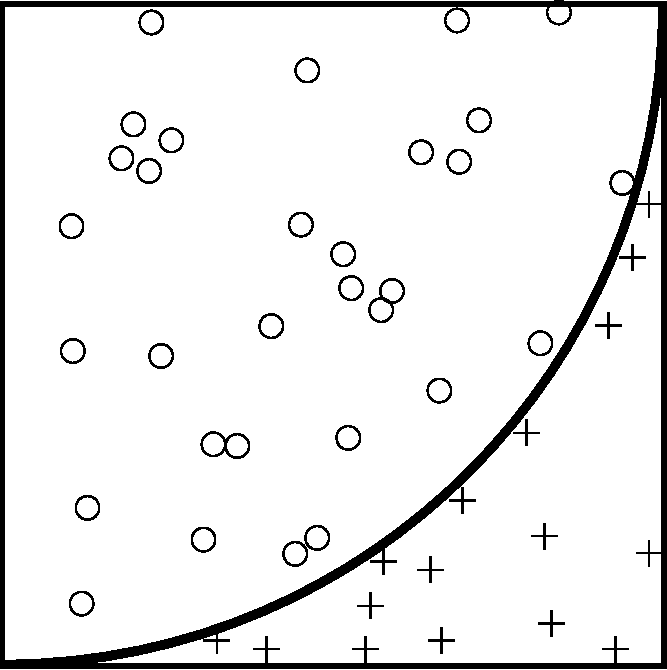
\includegraphics[scale=0.4]{monte_carlo.pdf}
\caption{Ćwiartka koła w kwadracie.}
\label{fig:awesome_image}
\end{figure}

\section*{Liczenie przybliżeń liczby \(\pi\) metodą Monte Carlo}
Koło wpisane w jednostkowy kwadrat ma powierzchnię równą  \(\pi/4\). Toteż losując punkty w kwadracie z prawdopodobieństwem  \(\pi/4\) trafiamy w obszar koła. 
Dzięki temu, zliczając odsetek wylosowanych punktów, które trafiły do wnętrza koła, możemy określić przybliżenie liczby   \(\pi\). Taka metoda zalicza się do metod Monte Carlo\footnote{w Monte Carlo mieści się bodaj najsłynniejsze w Europie kasyno, stąd taka nazwa dla metod losowych}. 

\subsection*{Ćwiczenia}
\begin{enumerate}
\item Przy użyciu poprzedniej funkcji policz przybliżenie liczby \(\pi\). Wykonaj 10000 losowań.
\item Sprawdź, jak zmienia się dokładność przybliżeń, gdy wykonujemy coraz więcej losowań. Wykonaj 100, 1000 i 100000  losowań. 
\item* Wydrukuj na ekran zależność względnego błędu przybliżenia \(\pi\) od potęgi liczby 2 w zakresie  \(2^{8}\) do \(2^{32}\).




\end{enumerate}

\end{document}
